% Dokumentenklasse
\documentclass{article}

% Pakete
\usepackage{tex/pakete}
\usepackage{tex/macros}

% Einstellen der Pakete
\graphicspath{{figs/}}
\addbibresource{refs.bib}
\titleformat{\section}
  {\normalfont\LARGE\bfseries}{\thesection.}{.3em}{}
\titlespacing*{\section}{0pt}{3.5ex plus 1ex minus .2ex}{2.3ex plus .2ex}
\titleformat{\subsection}
  {\normalfont\Large\bfseries}{\thesubsection.}{.3em}{}
\titlespacing*{\subsection}{0pt}{3.5ex plus 1ex minus .2ex}{2.3ex plus .2ex}
\titleformat{\subsubsection}
  {\normalfont\large\bfseries}{\thesubsubsection.}{.3em}{}
\titlespacing*{\subsubsection}{0pt}{3.5ex plus 1ex minus .2ex}{2.3ex plus .2ex}

\sisetup{output-decimal-marker = {,}}

%\numberwithin{equation}{section}

\pagestyle{fancy}
%\fancyhf{}
\lhead{P422 Rastertunnelmikroskopie}
\rhead{Gabriel Remiszewski und Christian Fischer}

% Titelblatt
\title{\textbf{Versuchsbericht} \\ \Large{\textbf{P422 Rastertunnelmikroskopie}}}
\date{durchgeführt am 2/3.11.2023}
\author{Gabriel Remiszewski und Christian Fischer}

%========================================================================
\begin{document}

\begin{titlepage}
\maketitle
\thispagestyle{empty}
\end{titlepage}
\newpage
\tableofcontents
\thispagestyle{empty}
\newpage

% "Einleitung"
\section{Einleitung}\label{sec:einleitung}
\pagenumbering{arabic}
\cite{skript}

% "Versuchsabschnitte"
\section{Bedienung des Rastertunnelmikroskops}\label{sec:versuch}
Bei der Versuchsdurchführung wird ein RTM mit einem externen Controller und der zugehörigen Software \texttt{Easyscan 2} verwendet.
Der Experimentierplatz ist in \cref{fig:versuchsplatz} gezeigt.
\begin{figure}[H]
	\centering
	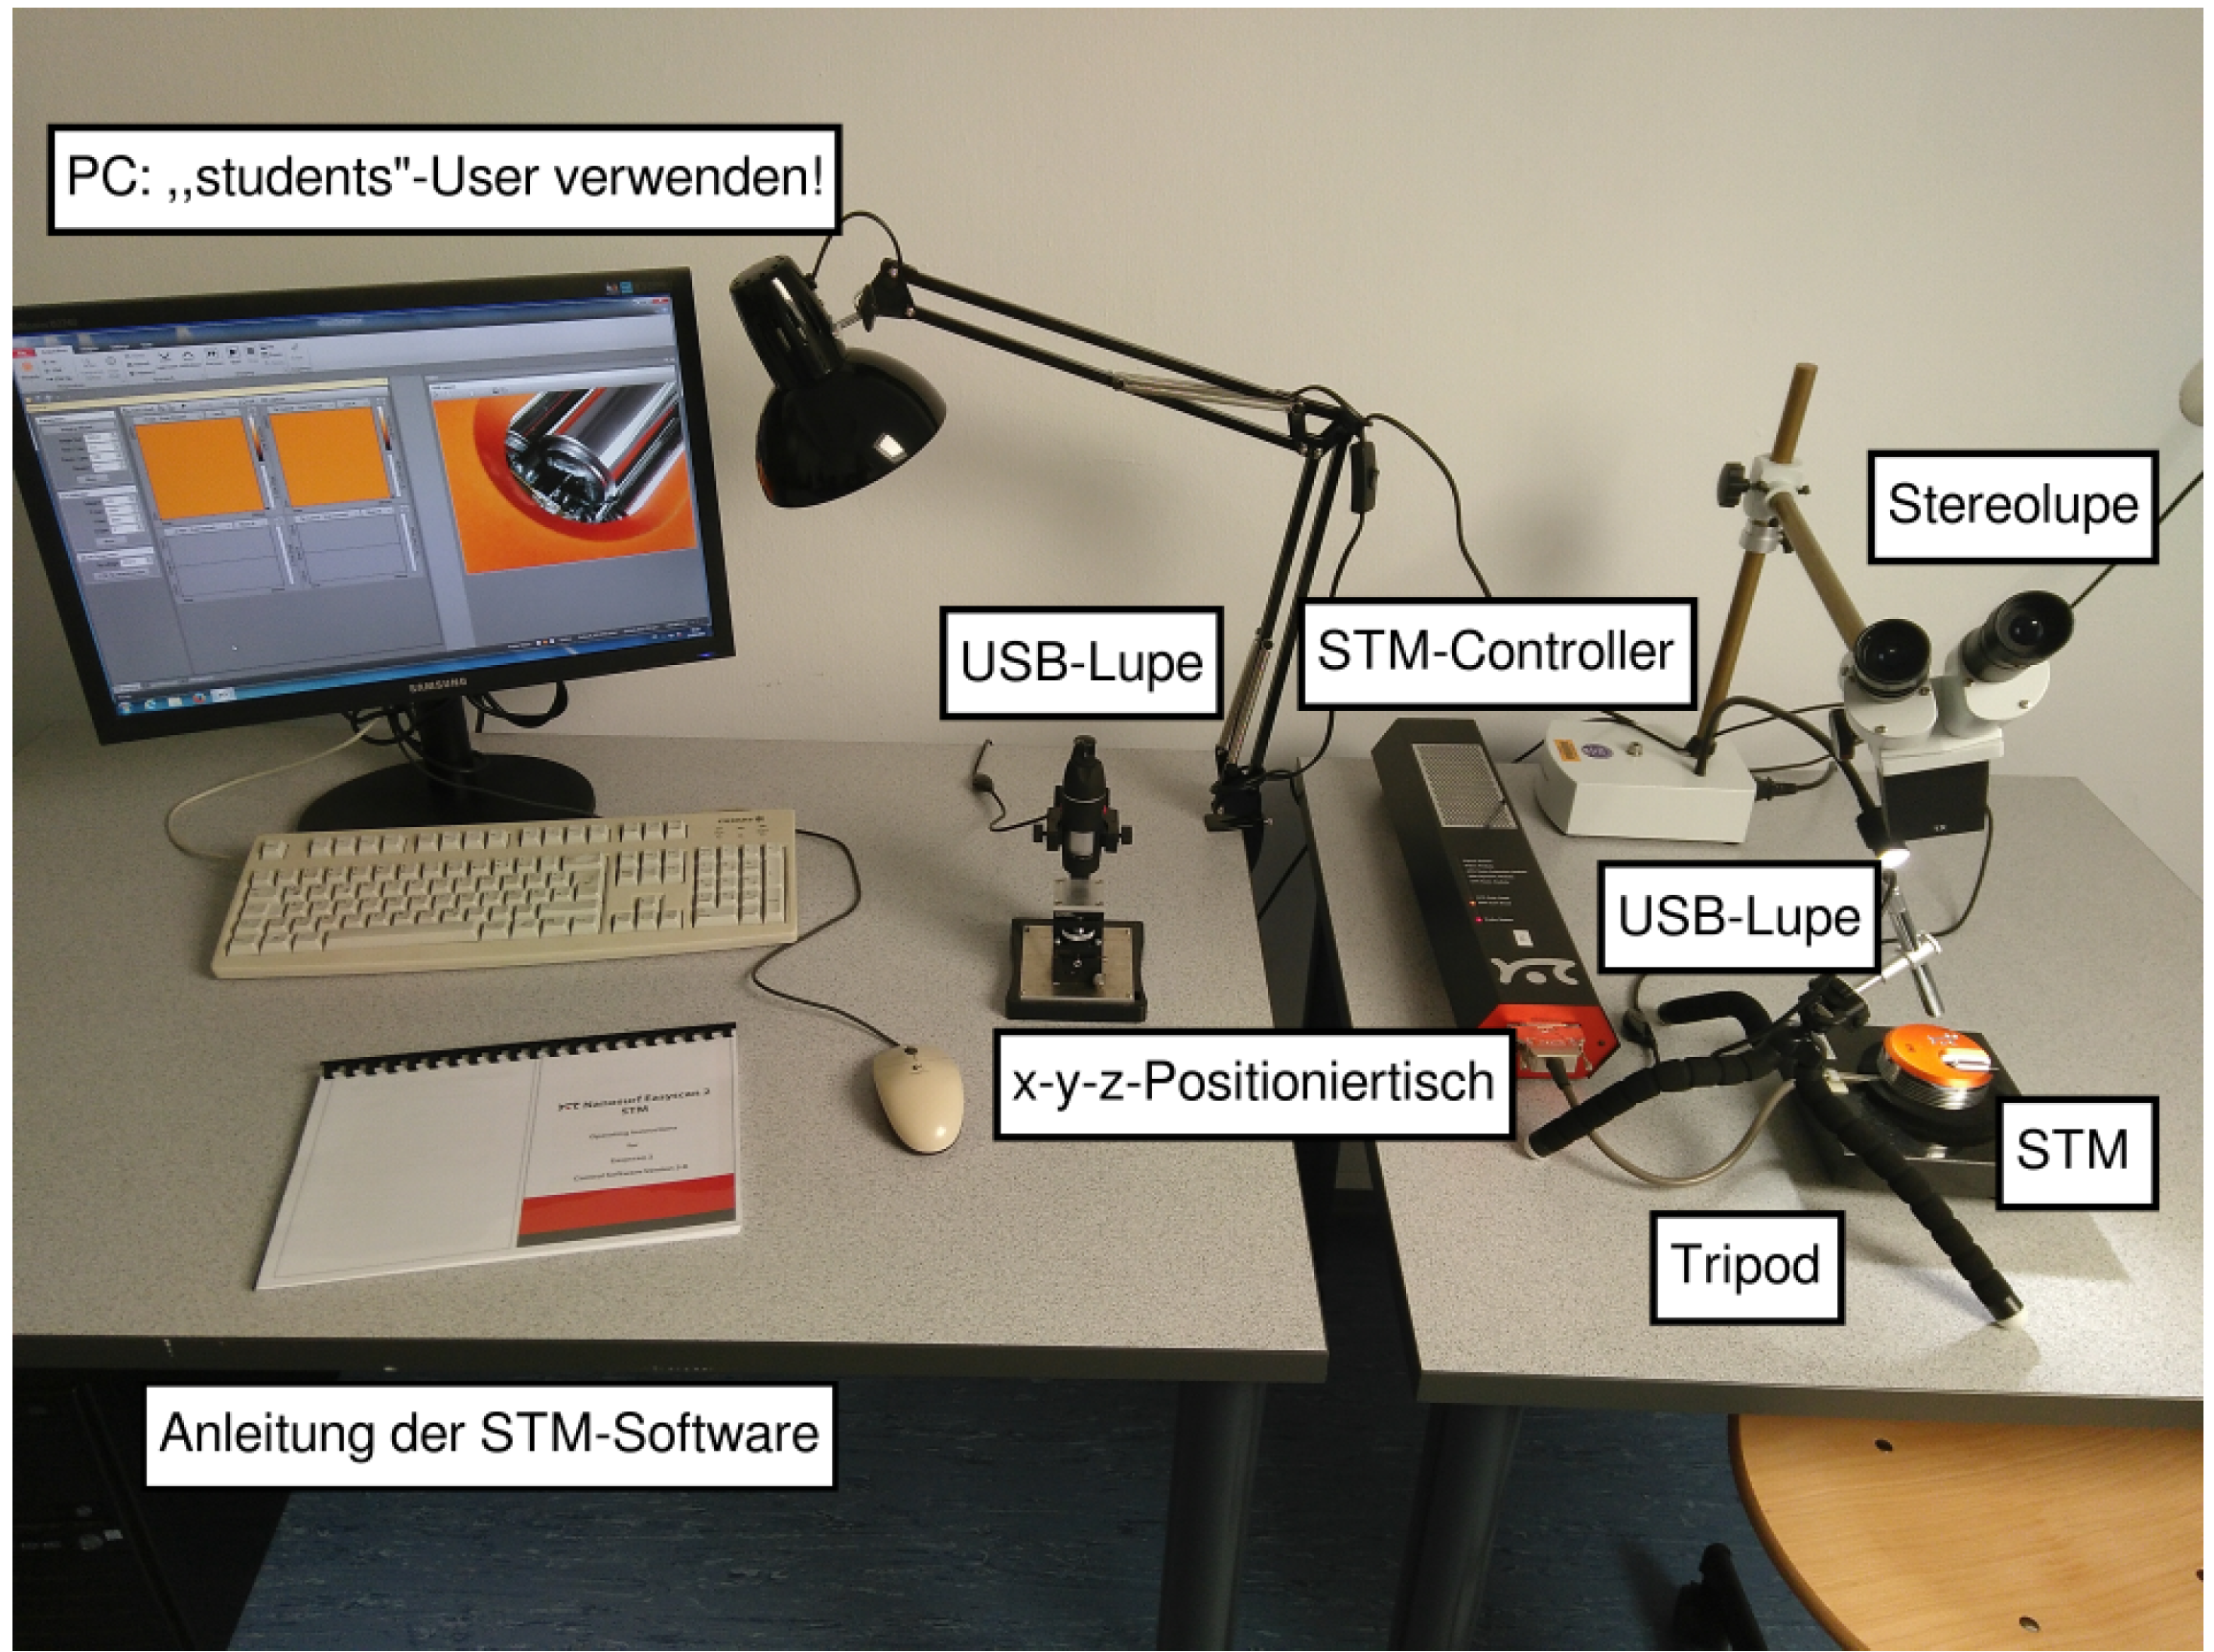
\includegraphics[width=0.8\linewidth]{../figs/versuchsplatz.png}
	\caption{Experimentierplatz mit RTM und dem notwendigen Zubehör (Quelle: \cite{skript})}
	\label{fig:versuchsplatz}
\end{figure}
Um mit dem RTM arbeiten zu können, wird der RTM-Controller über einen Kippschalter eingeschaltet. Anschließend wird der beistehende Rechner
hochgefahren, um die für den RTM-Controller benötigte Software \texttt{Easyscan 2} zu öffnen. Außerdem ist der Arbeitsbereich mit den Eingabegeräten
des Rechners (Tastatur und Maus) auf einem anderen Tisch als das RTM platziert, sodass die vielen Berührungspunkte der Hände, Arme, Füße und Beine mit dem Tisch während der Bedienung
der Software keinen Einfluss auf die Arbeitsweise des RTMs haben. Ohnehin ist das RTM auf einem schwingungsdämpfenden Körper befestigt, um
den Einfluss von Vibrationen auf die Messungen zu verringern, allerdings hat sich bei der Versuchsdurchführung tatsächlich gezeigt, dass leichte Zusammenstöße
mit dem RTM-Tisch zu kurzzeitigen Ausreißern während eines Messprozesses führen, weshalb eine Aufteilung der beteiligten Arbeitsgeräte definitv sinnvoll ist.\par
Auf dem Tisch mit dem Rechner ist zudem eine USB-Lupe positioniert, mit der die verwendeten Proben und Spitzen auf ihre Qualität untersucht werden können.
Für diese USB-Lupe wird eine separate Software verwendet.\par
Das RTM weißt eine Öffnung auf, in welche die Spitze und Probe eingesetzt werden können. Diese Öffnung ist mit einer Schutzkappe abgedeckt, welche aber für
die Versuchsdurchführung entfernt werden kann. Darüber hinaus wird eine weitere USB-Lupe (montiert auf einem Dreibein) auf die Öffnung des RTMs gerichtet,
um später die Annäherung der Probe an die Spitze beobachten zu können. Das resultierende Bild dieser USB-Lupe kann in \texttt{Easyscan 2} dargestellt werden.\par
Die Proben, der Spitzendraht und das benötigte Zubehör befindet sich in einer Box (siehe \cref{fig:koffer}).
\begin{figure}[H]
	\centering
	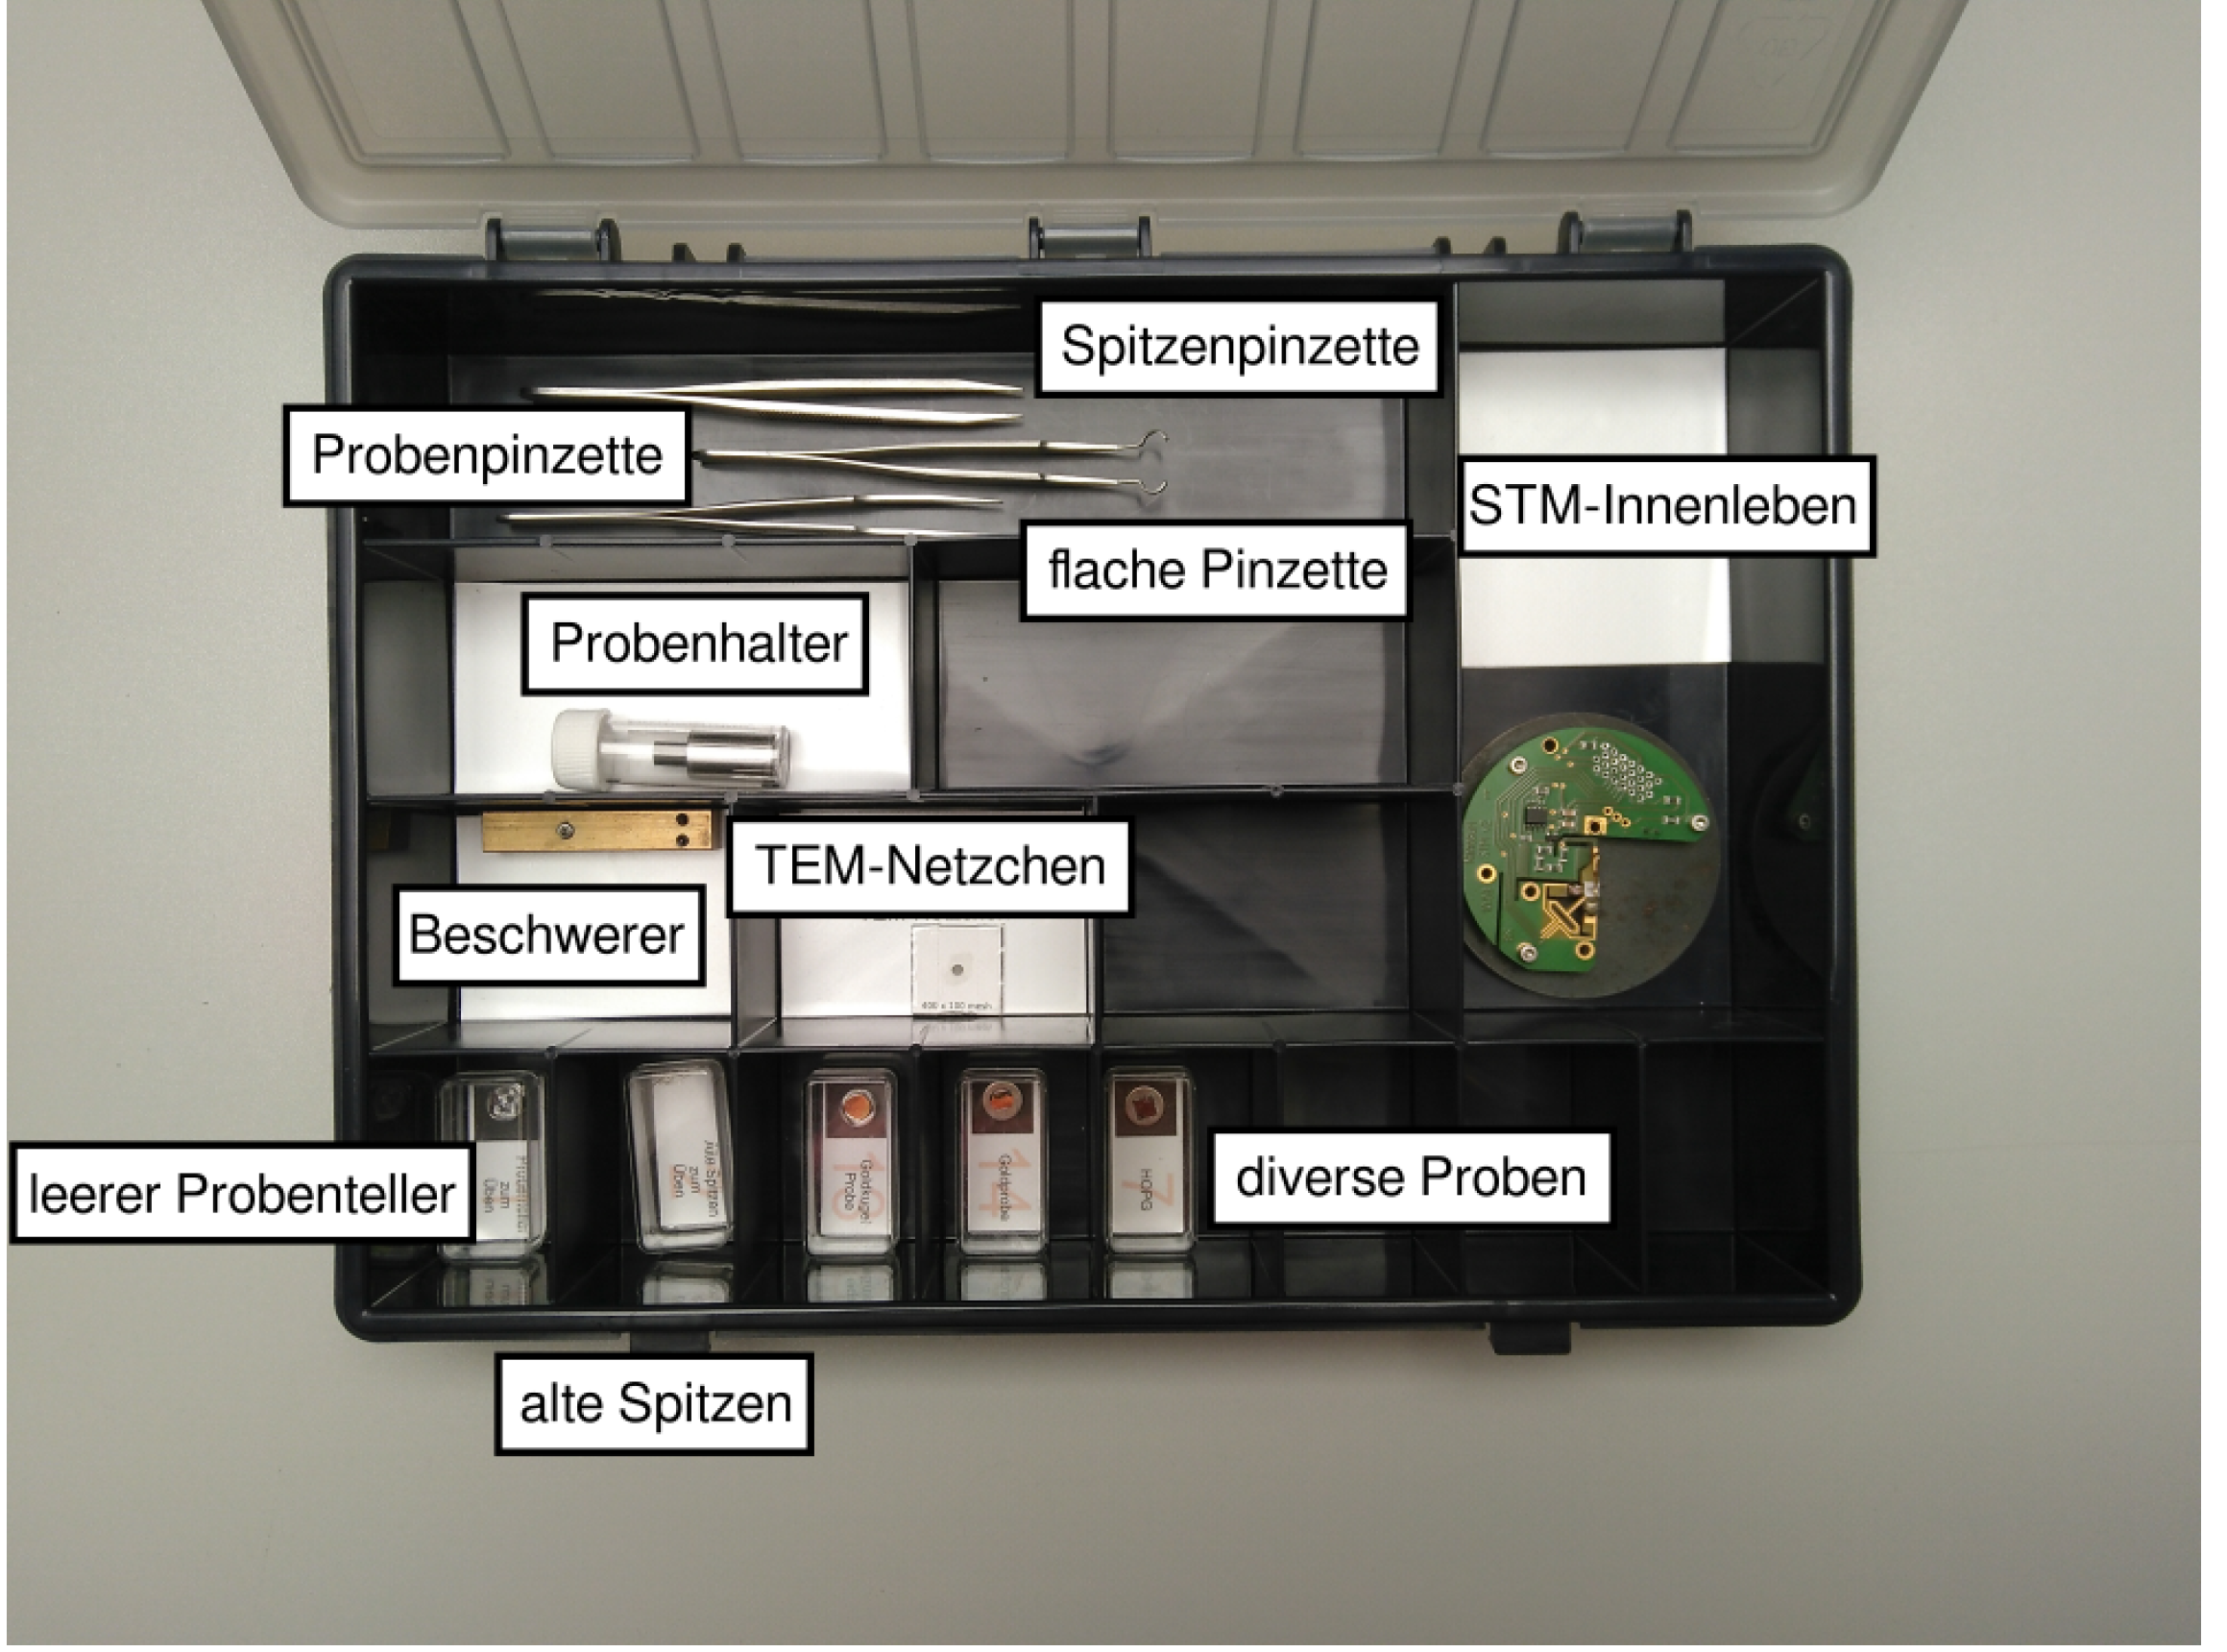
\includegraphics[width=0.8\linewidth]{../figs/koffer.png}
	\caption{Box mit den Proben und dem benötigten Zubehör (Quelle: \cite{skript})}
	\label{fig:koffer}
\end{figure}
\section{Gold-Probe}\label{sec:gold}
Um den Umgang mit dem zur Verfügung stehenden RTM zu erlernen, wird zunächst eine Gold-Probe (Gold auf Saphir) untersucht, da hier die vorkommenden groben Strukturen leicht
abzubilden sind. In einem ersten Schritt wird eine Messspitze mit einem Seitenschneider aus dem Platin-Iridium-Draht zugeschnitten. Hier wird darauf geachtet,
dass der Platin-Iridium-Draht an einer Seite möglichst spitz zugeschnitten wird. Um eine Oberfläche mit atomarer Auflösung abzubilden, ist es notwendig, dass
die Spitze einatomig ist. Zuerst scheint es etwas unrealistisch, einen Draht auf eine einatomige Spitze zuzuschneiden. Allerdings wird es in der Praxis
meist der Fall sein, dass die zugeschnittene Spitze einatomig ist, da es immer ein Atom gibt, was im Vergleich zu seinem Nachbaratom noch ein wenig weiter vorne ist.
Dies reicht bereits für eine atomare Auflösung aus, da der Abstand zwischen Spitze und Probe in der Größenordnung eines Atomdurchmessers liegt. Somit wird
ein Elektron immer zu dem einzelnen vordersten Atom der Spitze tunneln, da die Tunnelwahrscheinlichkeit zu einem leicht dahinter liegenden Atom exponentiell
mit dem Abstand (bereits ungefähr zwei Atomdurchmesser) abfällt.\par
Die zugeschnittene Spitze kann nun in dem RTM-Innenleben zur Betrachtung unter der USB-Lupe befestigt werden. Diese Spitze wird für die gesamte Untersuchung
der Gold-Probe verwendet. In Abbildung \cref{fig:spitze1} ist die verwendete Spitze dargestellt. Links ist der Zustand der Spitze vor und rechts nach der Untersuchung
der Gold-Probe abgebildet. Der \SI{0,3}{\milli \meter}-dicke Platin-Iridium wird zur Kalibrierung der eingezeichneten Maßstäbe verwendet.
\begin{figure}[H]
    \centering
    \begin{subfigure}{0.45\textwidth}
        \centering
        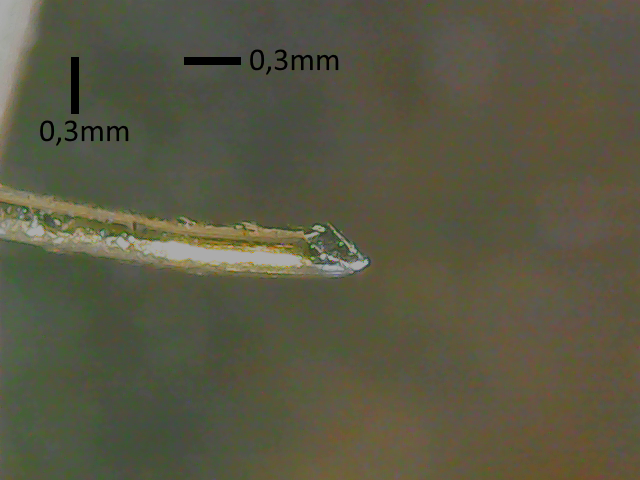
\includegraphics[width=\linewidth]{../figs/spitze1_vorher}
        \caption{vorher}
    \end{subfigure}
    \begin{subfigure}{0.45\textwidth}
        \centering
        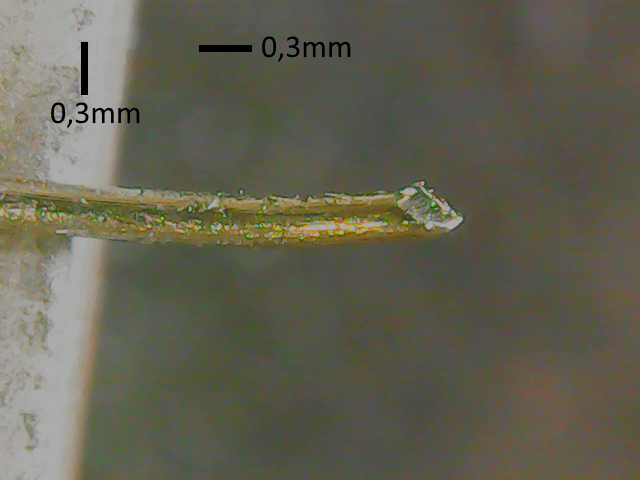
\includegraphics[width=\linewidth]{../figs/spitze1_nachher}
        \caption{nachher}
    \end{subfigure}
    \caption{Messspitze zur Untersuchung der Gold-Probe unter dem USB-Mikroskop}\label{fig:spitze1}
\end{figure} Mit dem USB-Mikroskop kann allerdings keine Aussage über die Qualität der Spitze getroffen werden. Es lässt sich auch nicht erkennen, ob
sich die Struktur der Spitze vorne während der Versuchsdurchführung maßgeblich verändert hat. Auch ist leider nicht zu erkennen, ob die Spitze
während der Versuchsdurchführung Dreck aufgesammelt hat, was unter anderem für schlechtere Messergebnisse gesorgt haben könnte.\par
Als Gold-Probe wird eine solche verwendet, bei der eine Goldschicht auf Saphir aufgetragen ist. Bevor diese Probe untersucht wird, wird
ihr Zustand mit dem USB-Mikroskop dokumentiert. Zur Kalibrierung des USB-Mikroskops wird ein $400 \times 100$-Mesh benutzt. Zur Kalibrierung werden
die \num{100} Mesh verwendet. Dies bedeutet, dass sich auf einem Zoll \num{100} Öffnungen befinden (vgl. \cite{mesh}). In \cref{fig:maßstab_gold} werden fünf solcher
Öffnungen abgezählt, womit die eingezeichnete Länge $\frac{5}{100} = \num{0,05}$ Zoll entspricht. Die Umrechnung in \unit{\milli \meter} wird durch eine
Multiplikation mit dem Faktor \num{25,4} vorgenommen (siehe \cite{umrechnung}).
\begin{figure}[H]
	\centering
	\includegraphics[width=0.8\linewidth]{../figs/maßstab_gold.png}
	\caption{$400 \times 100$-Mesh zur Kalibrierung des Maßstabes des USB-Mikroskops}
	\label{fig:maßstab_gold}
\end{figure}
\section{HOPG-Probe}\label{sec:hopg-probe}
\subsection*{Struktur}
Hochorientierter pyrolyitscher Graphit (HOPG) ist kristalliner Kohlenstoff, wo Atome einer Schicht
auf einem hexagonalen Gitter geordnet sind, wodurch jedes Atom auf dieser zweidimensionalen
Ebene von drei weiteren Atomen im Winkel von \SI{120}{\degree} verbunden ist. Zwei Schichten
dieses Gitters sind versetzt übereinander geordnet (siehe \cref{fig:hopg-skizze}), weshalb durch die
untere Ebene die Ladungsverteilung auf der Oberfläche beeinflusst wird.\par Wie in
\cref{fig:hopg2} erkennbar ist bei den H-Atomen die Ladungsverteilung minimal und bei A-Atomen maximal.
Die Verteilung bei den B-Atomen befindet sich dazwischen, weshalb diese für das Mikroskop unsichtbar werden,
da ein RTM nicht unmittelbar die Oberflächentopographie messen kann, sondern die Aufenthaltswahrscheinlichkeit der
Elektronen \cite[Kap.1 S.7]{rtm-leitpfaden}.

\begin{figure}[htb]
	\centering
	\begin{subfigure}{0.45\linewidth}
		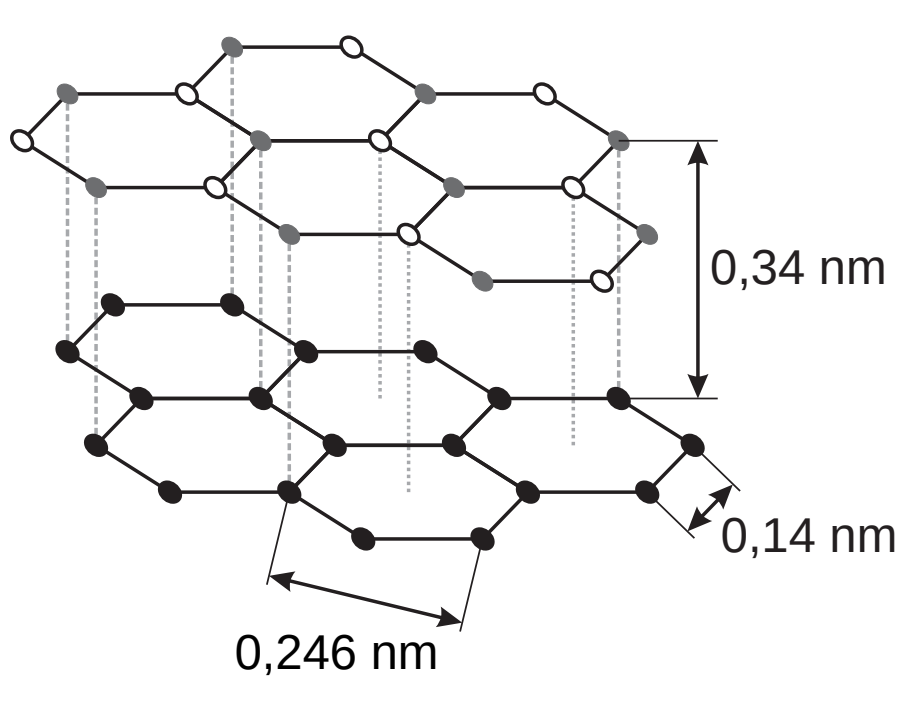
\includegraphics[width=\linewidth]{figs/hopg1.png}
		\caption{Seitenansicht.\cite[S.49]{skript}}
		\label{fig:hopg1}
	\end{subfigure}
	\hspace{0.5cm}
	\begin{subfigure}{0.45\linewidth}
		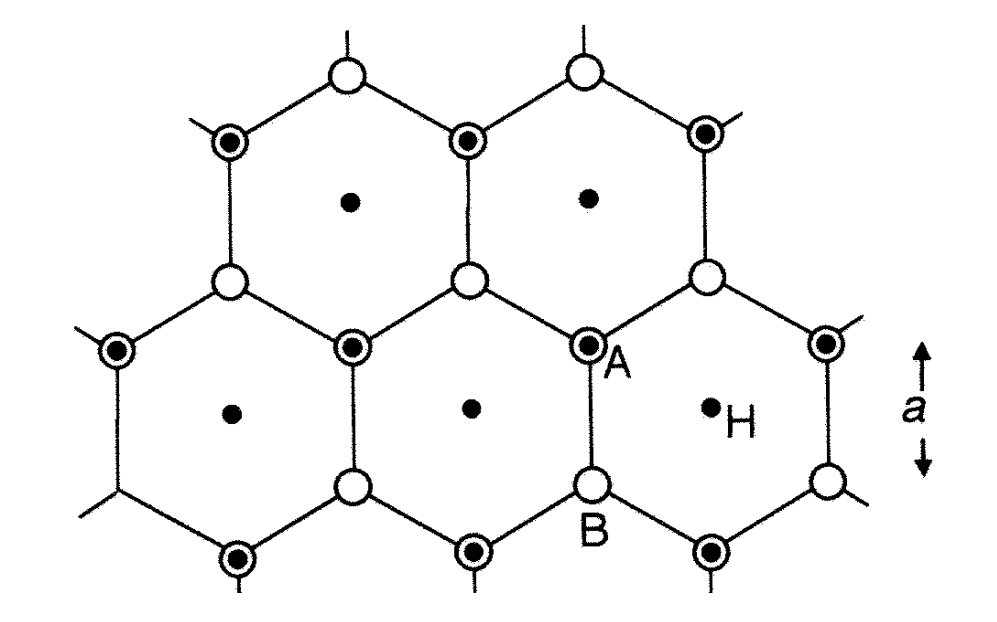
\includegraphics[width=\linewidth]{figs/hopg2.png}
		\caption{Obere Ansicht.\cite[Kap.1 S.17]{rtm-leitpfaden}}
		\label{fig:hopg2}
	\end{subfigure}
	\caption{Hochorientierter pyrolyitscher Graphit.}
	\label{fig:hopg-skizze}
\end{figure}

\subsection*{Vorbereitung}
Im Gegensatz zu Gold wird hier versucht, die atomare Struktur des Graphits aufzulösen.
Dies erfordert hohe Präzision in der Durchführung und der Präparierung der Spitze. Der Platin-Iridium Draht
vor der Rasterung ist in \cref{fig:spitze_hopg_vorher_v2} abgebildet. Vorne ist eine dünne Spitze zur ekennen,
die sich für die Durchführung eignen sollte.

\begin{figure}[htb]
	\centering
	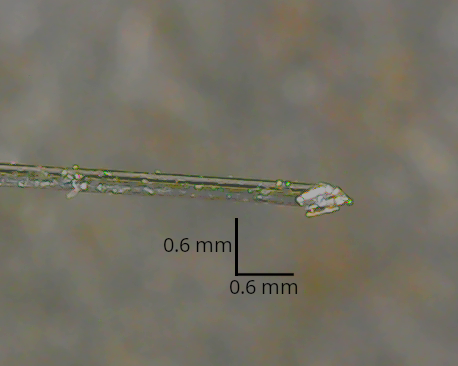
\includegraphics[width=0.5\linewidth]{figs/spitze_hopg_vorher_v2.png}
	\caption{Platin-Iridium Spitze vor Rasterung des HOPG.}
	\label{fig:spitze_hopg_vorher_v2}
\end{figure}

Die Graphit-Probe ist in \cref{fig:usb_mikroskop_hopg} mit zwei unterschiedlichen
Vergrößerungen abgebildet. Zu erkennen ist eine Stufenstruktur auf der Obefläche, die jedoch
deutlich größer ist als die Fläche, die gerastert werden soll. Daher kann mit dieser
Probe gearbeitet werden.


\begin{figure}[htb]
	\centering
	\begin{subfigure}{0.45\linewidth}
		\centering
		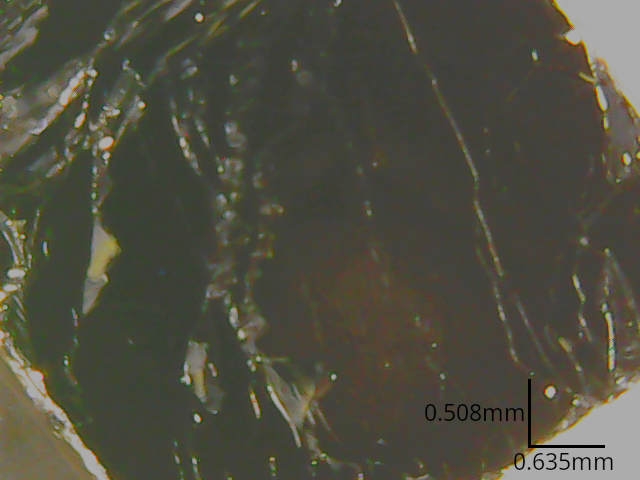
\includegraphics[width=\linewidth]{figs/hopg_skala1.png}
		\caption{Skala 1}
		\label{fig:hopg_skala1}
	\end{subfigure}
	\hspace{0.5cm}
	\begin{subfigure}{0.45\linewidth}
		\centering
		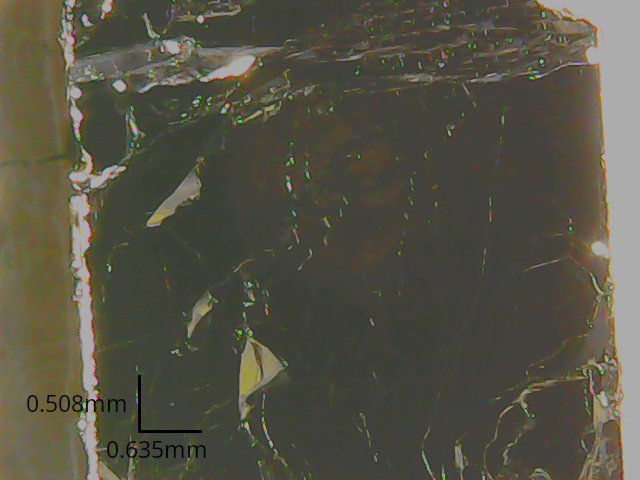
\includegraphics[width=\linewidth]{figs/hopg_skala2.png}
		\caption{Skala 2}
		\label{fig:hopg_skala2}
	\end{subfigure}
	\caption{USB-Mikroskop Aufnahmen von HOPG nach Abziehen der obersten Schicht.}
	\label{fig:usb_mikroskop_hopg}
\end{figure}

\subsection*{Auswertung}

Nach erfolgreicher Annäherung der Probe an die Spitze wird zunächst ein Bild
mit einer großen Breite gemacht, um die Grobstruktur der Oberfläche
zu bekommen um damit einen ausreichend flachen Flächenabschnitt
finden zu können. Ein Bild bei einer Breite von $\SI{200}{\nm}$ ist in 
\cref{fig:hopg_rtm_weitaufnahme} zu sehen, wobei das oben rechte Viertel 
von einer flachen Ebene gefüllt wird, wo die Höhe nur um einen Atomdurchmesser schwankt.

\begin{figure}[htb]
	\centering
	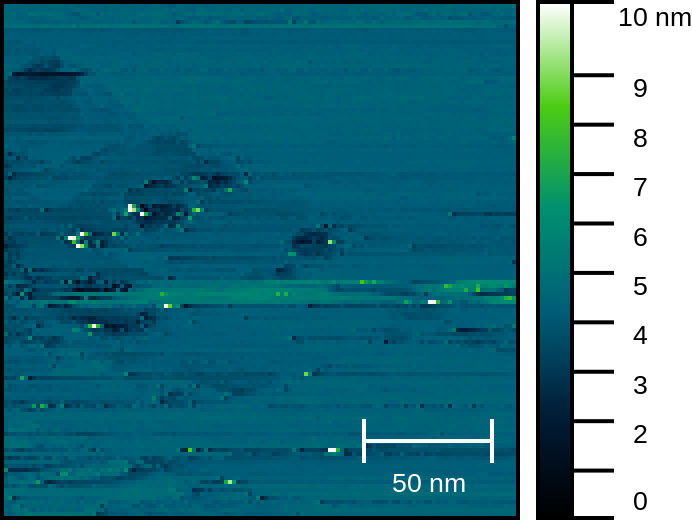
\includegraphics[width=0.6\linewidth]{figs/HOPG10558.png}
	\caption{$I_\mathrm{set}=\SI{5}{\nm}$, $V=\SI{500}{\milli\volt}$, $P=1000$, $I=2000$,
		$v=\SI{1}{\nm\per\s}$}
	\label{fig:hopg_rtm_weitaufnahme}
\end{figure}



% "Fazit"
\section{Fazit}\label{sec:fazit}
Mithilfe der Bragg-Reflexion konnte von zwei unterschiedlichen Anoden einer 
Röntgenröhre die K$_\alpha$ und K$_\beta$ Linien der charakteristischen 
Röntenstrahlung untersucht werden. Die Wellenlängen multipliziert mit der Beugungsordnung 
der Anode aus einem zuvor unbekannten Element sind in \cref{tab:anode-unbekannt}
vorzufinden. Dabei konnte festgestellt werden, dass sämtliche 
Linien Vielfache der ersten beiden Linien (vom Diagramm aus links gesehen)
darstellen, womit schlussgefolgert werden kann, dass die hier beobachteten Linien
zwei charakeristische Linien bis zur vierten Beugungsordnung darstellen solllen.
Das unbekannte Element konnte als Silber identifiziert werden, da 
dessen Spektrum eine K$_\beta$-Linie bei \SI{49.3}{\pm} aufweist und der 
Messwert von \SI{49.26\pm0.06}{\pm} im $1\sigma$-Bereich der Messung liegt. Eine K$_\alpha$ 
Linie liegt bei \SI{55.942}{\pm}, während eine Wellenlänge von \SI{55.63\pm0.05}{\pm}
gemessen werden konnte. Da die erste Linie mit der Literatur übereinstimmt, ist eine 
Abweichung bei der zweiten Linien ungewöhnlich. Eine Verschiebung 
des Kristalls während der Messung könnte Ursache für die Diskrepanz sein.\par 
Von einer Molybdän-Anode wurde zusätzlich die Feinstrukturaufspaltung 
der K$_\alpha$-Linie in der vierten Beugungsordnung gemessen, was in \cref{fig:feinstruktur}
zu sehen ist. In \cref{tab:feinstruktur} sind die gemessenen 
Energien im Vergleich zu den Literaturwerten zu sehen. Dabei konnte die Feinstrukturaufspaltung
auf drei signifikante Stellen genau gemessen werden, da jedoch die in diesem Versuch 
abgeschätzten Fehler deutlich kleiner sind, liegen die Referenzwerte nicht im $3\sigma$-Bereich
der Messung. Dies ist auch für Wellenlängendifferenz
\begin{equation*}
	\Delta\lambda_\mathrm{Exp} = \SI{0.444\pm 0.008}{\pm},\qquad
	\Delta\lambda_\mathrm{Ref} = \SI{0.428\pm0.004}{\pm}
\end{equation*}
zu beobachten, weshalb ein systematischer Fehler als Ursache für die Abweichung 
ausgeschlossen wird. Eine leichte Verschiebung des Kristalls stellt dabei 
eine realistische Fehlerquelle dar.\\\par

Mit der Röntgenfluoreszenz konnte die Zusammensetzung von 
Legierungen analysiert werden. Hierfür wurden mit verschiedenen metallischen Plätchen 
das dazugehörige Röntegenspektrum durch Fluoreszenz gemessen werden. Nach Kallibration
der Messung durch den Vielkanalanalysator konnte dem Spektrum Energien zugegeordnet werden und die 
Intensitäten der Linien konnten mit den Intensitäten der Legierungen verglichen werden und somit
die Massenanteile der Elemente. Hierbei konnte die zweite Legierung als 
Mischung von Kupfer und Zink identifiziert werden mit, im Fehlerbereich, gleichen Anteilen von 
\begin{equation*}
    C_\mathrm{Cu} = 49.6(5)\%,\quad C_\mathrm{Zn} = 50(2)\%.
\end{equation*}
Einen Vergleichswert hierzu gibt es nicht, weshalb eine quantitative Einordnung der Messwerte 
nicht möglich ist. Der Wert liegt jedoch in realistischen Bereichen.
\\\par

Im dritten Versuchsteil wurde die Symmetrie und Gitterstruktur eines NaCl-Kristalls mithilfe des Laue-Verfahrens
untersucht. Dazu wurde der zu untersuchende NaCl-Kristall über \SI{1800}{\second} mit von einer
Molybdän-Röntgenröhre erzeugten Röntgenstrahlung belichtet. Die Röntgenstrahlung wird teilweilse durch den
NaCl-Kristall transmittiert und teilweise an den unterschiedlichen Netzebenenscharen gebeugt. Hinter dem Kristall
wird die transmittierte und gebeugte Röntgenstrahlung mithilfe eines Röntgenfilms nachgewiesen, welcher nach
einer Entwicklung zur Auswertung bereit steht.\par
Ziel der Auswertung war es, die einzelnen Reflexe auf dem Röntgenfilm mit den entsprechenden Millerschen Indizes
zu identifizieren, welche die Orientierung der einzelnen Netzebenenscharen beschreiben. So konnte rausgefunden werden,
welche Netzebenenscharen des NaCl-Kristalls für welchen Reflex verantwortlich waren. Die Zuordnung der Millerschen
Indizes stellte hier eine Herausforderung da, da das Reflexmuster auf dem Röntgenfilm gewölbt war. Dennoch konnte
die Zuordnung unter Berücksichtung der Symmetrie des NaCl-Kristalls (kubische Symmetrie) erfolgreich durchgeführt werden.
Die Ergebnisse sind in \cref{tab:miller2} zu finden.\par
Anschließend konnten mit den Millerschen Indizes der Netzebenenabstand der einzelnen Netzebenen einer Netzebenenschar,
der Glanzwinkel und die für einen Reflex verantwortlichen Wellenlängen (es tragen mehrere Beugungsordnungen bei)
bestimmt werden. Die berechneten Werte sind in \cref{tab:keineahnung} einzusehen.

% "Anhang"
\appendix
\section*{Anhang}\label{sec:anhang}


% Literaturverzeichnis ausgeben
\printbibliography[heading=bibintoc, title = {Literaturverzeichnis}]

\end{document}
%========================================================================